% This file is generated by the MATLAB m-file laprint.m. It can be included
% into LaTeX documents using the packages graphicx, color and psfrag.
% It is accompanied by a postscript file. A sample LaTeX file is:
%    \documentclass{article}\usepackage{graphicx,color,psfrag}
%    \begin{document}% This file is generated by the MATLAB m-file laprint.m. It can be included
% into LaTeX documents using the packages graphicx, color and psfrag.
% It is accompanied by a postscript file. A sample LaTeX file is:
%    \documentclass{article}\usepackage{graphicx,color,psfrag}
%    \begin{document}% This file is generated by the MATLAB m-file laprint.m. It can be included
% into LaTeX documents using the packages graphicx, color and psfrag.
% It is accompanied by a postscript file. A sample LaTeX file is:
%    \documentclass{article}\usepackage{graphicx,color,psfrag}
%    \begin{document}% This file is generated by the MATLAB m-file laprint.m. It can be included
% into LaTeX documents using the packages graphicx, color and psfrag.
% It is accompanied by a postscript file. A sample LaTeX file is:
%    \documentclass{article}\usepackage{graphicx,color,psfrag}
%    \begin{document}\input{homocomp}\end{document}
% See http://www.mathworks.de/matlabcentral/fileexchange/loadFile.do?objectId=4638
% for recent versions of laprint.m.
%
% created by:           LaPrint version 3.16 (13.9.2004)
% created on:           20-Feb-2012 16:13:47
% eps bounding box:     15 cm x 11.25 cm
% comment:              
%
\begin{psfrags}%
\psfragscanon%
%
% text strings:
\psfrag{s06}[t][t]{\color[rgb]{0,0,0}\setlength{\tabcolsep}{0pt}\begin{tabular}{c}$M$\end{tabular}}%
\psfrag{s10}[][]{\color[rgb]{0,0,0}\setlength{\tabcolsep}{0pt}\begin{tabular}{c} \end{tabular}}%
\psfrag{s11}[][]{\color[rgb]{0,0,0}\setlength{\tabcolsep}{0pt}\begin{tabular}{c} \end{tabular}}%
\psfrag{s12}[l][l]{\color[rgb]{0,0,0}quasi-bicubic}%
\psfrag{s13}[l][l]{\color[rgb]{0,0,0}bilinear}%
\psfrag{s14}[l][l]{\color[rgb]{0,0,0}bicubic}%
\psfrag{s15}[l][l]{\color[rgb]{0,0,0}Collatz-Keys}%
\psfrag{s16}[l][l]{\color[rgb]{0,0,0}quasi-bicubic}%
%
% xticklabels:
\psfrag{x01}[t][t]{$32$}%
\psfrag{x02}[t][t]{$64$}%
\psfrag{x03}[t][t]{$128$}%
\psfrag{x04}[t][t]{$256$}%
\psfrag{x05}[t][t]{$512$}%
\psfrag{x06}[t][t]{$1024$}%
%
% yticklabels:
\psfrag{v01}[r][r]{$10^{-10}$}%
\psfrag{v02}[r][r]{$10^{-5}$}%
%
% Figure:
\resizebox{0.5\columnwidth}{!}{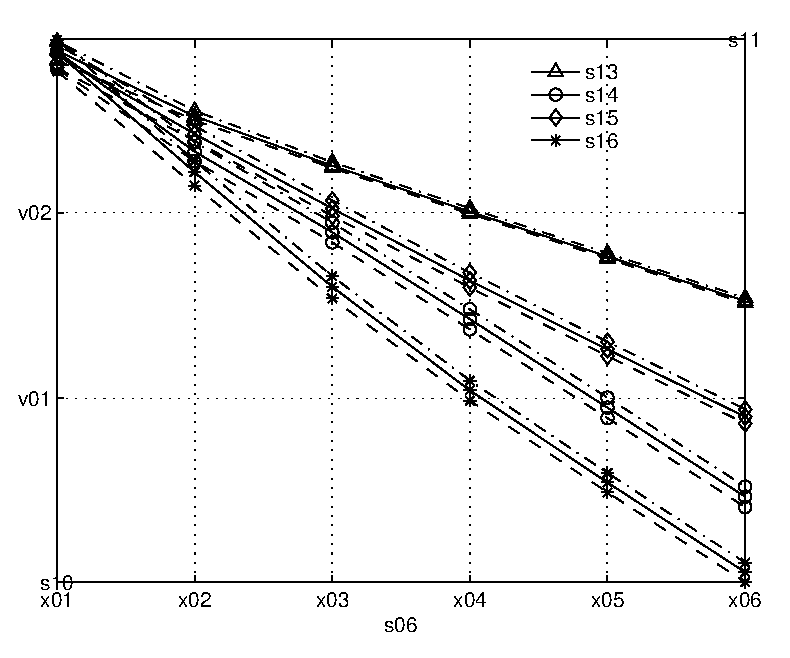
\includegraphics{./files/chap4/figures/homocomp.eps}}%
\end{psfrags}%
%
% End homocomp.tex
\end{document}
% See http://www.mathworks.de/matlabcentral/fileexchange/loadFile.do?objectId=4638
% for recent versions of laprint.m.
%
% created by:           LaPrint version 3.16 (13.9.2004)
% created on:           20-Feb-2012 16:13:47
% eps bounding box:     15 cm x 11.25 cm
% comment:              
%
\begin{psfrags}%
\psfragscanon%
%
% text strings:
\psfrag{s06}[t][t]{\color[rgb]{0,0,0}\setlength{\tabcolsep}{0pt}\begin{tabular}{c}$M$\end{tabular}}%
\psfrag{s10}[][]{\color[rgb]{0,0,0}\setlength{\tabcolsep}{0pt}\begin{tabular}{c} \end{tabular}}%
\psfrag{s11}[][]{\color[rgb]{0,0,0}\setlength{\tabcolsep}{0pt}\begin{tabular}{c} \end{tabular}}%
\psfrag{s12}[l][l]{\color[rgb]{0,0,0}quasi-bicubic}%
\psfrag{s13}[l][l]{\color[rgb]{0,0,0}bilinear}%
\psfrag{s14}[l][l]{\color[rgb]{0,0,0}bicubic}%
\psfrag{s15}[l][l]{\color[rgb]{0,0,0}Collatz-Keys}%
\psfrag{s16}[l][l]{\color[rgb]{0,0,0}quasi-bicubic}%
%
% xticklabels:
\psfrag{x01}[t][t]{$32$}%
\psfrag{x02}[t][t]{$64$}%
\psfrag{x03}[t][t]{$128$}%
\psfrag{x04}[t][t]{$256$}%
\psfrag{x05}[t][t]{$512$}%
\psfrag{x06}[t][t]{$1024$}%
%
% yticklabels:
\psfrag{v01}[r][r]{$10^{-10}$}%
\psfrag{v02}[r][r]{$10^{-5}$}%
%
% Figure:
\resizebox{0.5\columnwidth}{!}{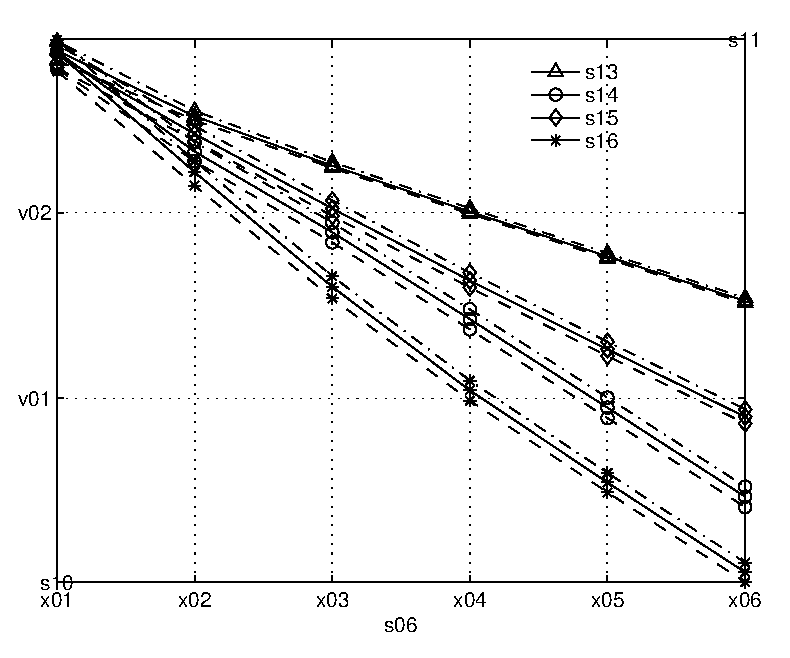
\includegraphics{./files/chap4/figures/homocomp.eps}}%
\end{psfrags}%
%
% End homocomp.tex
\end{document}
% See http://www.mathworks.de/matlabcentral/fileexchange/loadFile.do?objectId=4638
% for recent versions of laprint.m.
%
% created by:           LaPrint version 3.16 (13.9.2004)
% created on:           20-Feb-2012 16:13:47
% eps bounding box:     15 cm x 11.25 cm
% comment:              
%
\begin{psfrags}%
\psfragscanon%
%
% text strings:
\psfrag{s06}[t][t]{\color[rgb]{0,0,0}\setlength{\tabcolsep}{0pt}\begin{tabular}{c}$M$\end{tabular}}%
\psfrag{s10}[][]{\color[rgb]{0,0,0}\setlength{\tabcolsep}{0pt}\begin{tabular}{c} \end{tabular}}%
\psfrag{s11}[][]{\color[rgb]{0,0,0}\setlength{\tabcolsep}{0pt}\begin{tabular}{c} \end{tabular}}%
\psfrag{s12}[l][l]{\color[rgb]{0,0,0}quasi-bicubic}%
\psfrag{s13}[l][l]{\color[rgb]{0,0,0}bilinear}%
\psfrag{s14}[l][l]{\color[rgb]{0,0,0}bicubic}%
\psfrag{s15}[l][l]{\color[rgb]{0,0,0}Collatz-Keys}%
\psfrag{s16}[l][l]{\color[rgb]{0,0,0}quasi-bicubic}%
%
% xticklabels:
\psfrag{x01}[t][t]{$32$}%
\psfrag{x02}[t][t]{$64$}%
\psfrag{x03}[t][t]{$128$}%
\psfrag{x04}[t][t]{$256$}%
\psfrag{x05}[t][t]{$512$}%
\psfrag{x06}[t][t]{$1024$}%
%
% yticklabels:
\psfrag{v01}[r][r]{$10^{-10}$}%
\psfrag{v02}[r][r]{$10^{-5}$}%
%
% Figure:
\resizebox{0.5\columnwidth}{!}{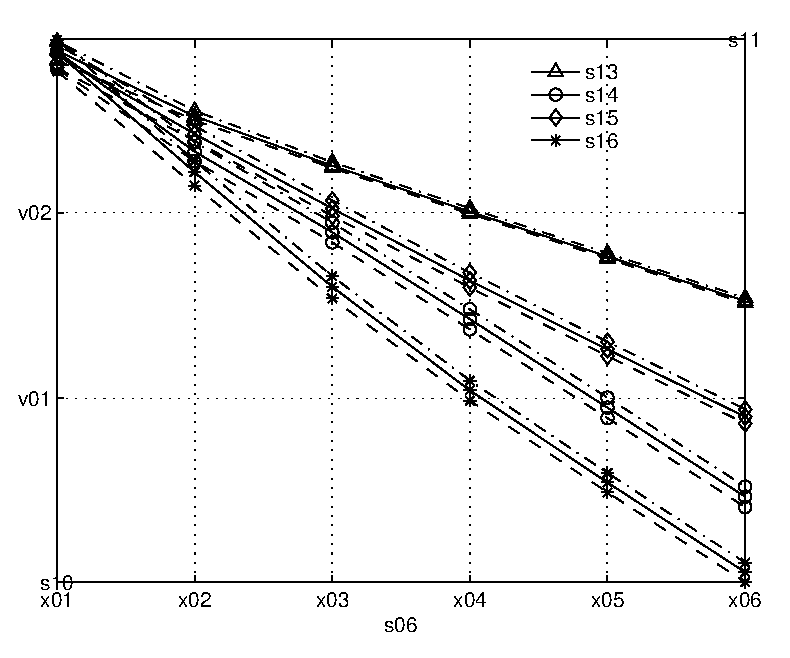
\includegraphics{./files/chap4/figures/homocomp.eps}}%
\end{psfrags}%
%
% End homocomp.tex
\end{document}
% See http://www.mathworks.de/matlabcentral/fileexchange/loadFile.do?objectId=4638
% for recent versions of laprint.m.
%
% created by:           LaPrint version 3.16 (13.9.2004)
% created on:           20-Feb-2012 16:13:47
% eps bounding box:     15 cm x 11.25 cm
% comment:              
%
\begin{psfrags}%
\psfragscanon%
%
% text strings:
\psfrag{s06}[t][t]{\color[rgb]{0,0,0}\setlength{\tabcolsep}{0pt}\begin{tabular}{c}$M$\end{tabular}}%
\psfrag{s10}[][]{\color[rgb]{0,0,0}\setlength{\tabcolsep}{0pt}\begin{tabular}{c} \end{tabular}}%
\psfrag{s11}[][]{\color[rgb]{0,0,0}\setlength{\tabcolsep}{0pt}\begin{tabular}{c} \end{tabular}}%
\psfrag{s12}[l][l]{\color[rgb]{0,0,0}quasi-bicubic}%
\psfrag{s13}[l][l]{\color[rgb]{0,0,0}bilinear}%
\psfrag{s14}[l][l]{\color[rgb]{0,0,0}bicubic}%
\psfrag{s15}[l][l]{\color[rgb]{0,0,0}Collatz-Keys}%
\psfrag{s16}[l][l]{\color[rgb]{0,0,0}quasi-bicubic}%
%
% xticklabels:
\psfrag{x01}[t][t]{$32$}%
\psfrag{x02}[t][t]{$64$}%
\psfrag{x03}[t][t]{$128$}%
\psfrag{x04}[t][t]{$256$}%
\psfrag{x05}[t][t]{$512$}%
\psfrag{x06}[t][t]{$1024$}%
%
% yticklabels:
\psfrag{v01}[r][r]{$10^{-10}$}%
\psfrag{v02}[r][r]{$10^{-5}$}%
%
% Figure:
\resizebox{0.5\columnwidth}{!}{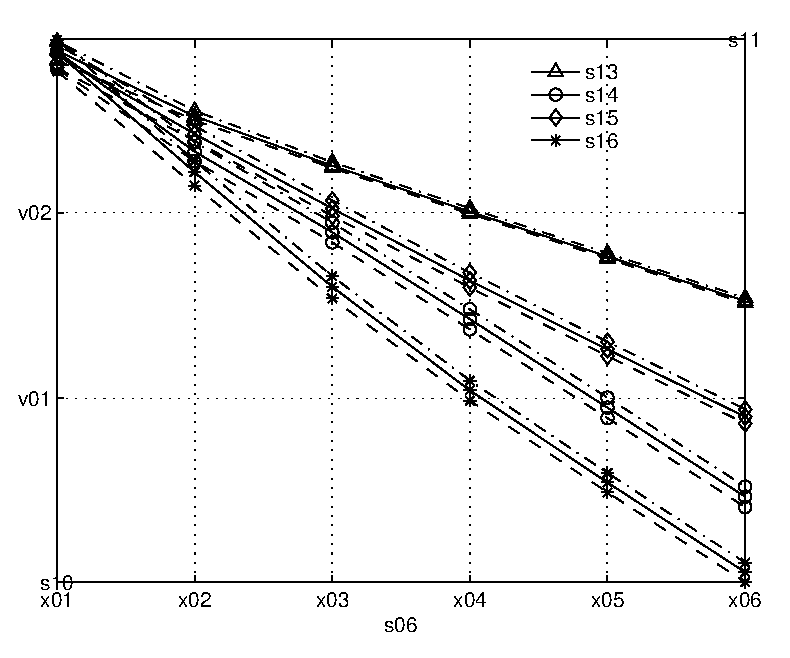
\includegraphics{./files/chap4/figures/homocomp.eps}}%
\end{psfrags}%
%
% End homocomp.tex
